\chapter{Discussion}
Please tell more about conclusion and how to the next work of this study.

\section{Imron Sumadireja / 1164076}
\subsection{Teori}
\begin{enumerate}
\item Jelaskan kenapa file teks harus dilakukan tokenizer. Dilengkapi dengan ilustrasi atau gambar \par
Tokenizer merupakan proses membagi teks yang dapat berupa kalimat, paragraf atau dokumen menjadi kata-kata atau bagian-bagian tertentu dalam kalimat tersebut. Sebagai contoh dari kalimat `Aku mau istirahat dulu ya untuk hari ini', menjadi `Aku', `Mau', `'Istirahat',`Dulu',`Ya',`Untuk',`Hari',`Ini'. Yang menjadi acuan yakni tanda baca dan spasi. Untuk ilustrasinya bisa dilihat pada gambar \ref{toke1}
		\begin{figure}[!htbp]
		\centerline{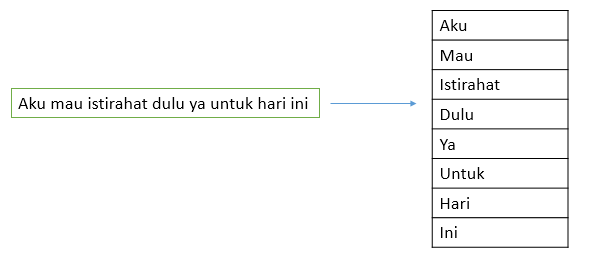
\includegraphics[width=0.5\textwidth]{figures/im/toke1.png}}
		\caption{Ilustrasi Tokenizer.}
		\label{toke1}
		\end{figure}

\item Jelaskan konsep dasar K Fold Cross Validation pada dataset komentar Youtube pada kode listing 7.1.dilengkapi dengan ilustrasi atau gambar \par
\lstinputlisting[firstline=1, lastline=2]{src/ron/tujuh.py}
Pada code tesebut terdapat kfold yang bertujuan untuk melakukan split data menjadi 5 bagian dari dataset komentar Youtube tersebut. Sehingga dari setiap data yang sudah dibagi tersebut akan menghasilkan presentase dari setiap bagiannya, untuk menghasilkan hasil akhir dengan presentase yang cukup baik. Untuk ilustrasi sederhananya bisa dilihat pada gambar \ref{toke2}
		\begin{figure}[!htbp]
		\centerline{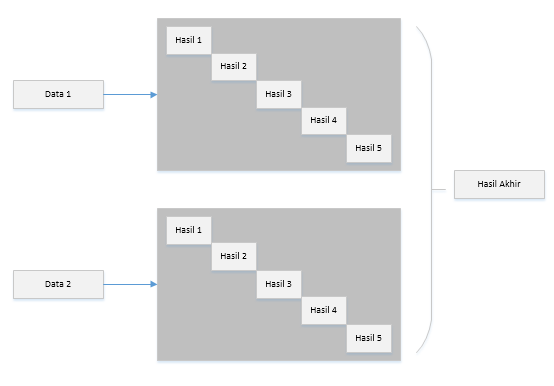
\includegraphics[width=0.5\textwidth]{figures/im/toke2.png}}
		\caption{Ilustrasi K-Fold Cross Validation.}
		\label{toke2}
		\end{figure}

\item Jelaskan apa maksudnya kode program for train, test in splits. Dilengkapi dengan ilustrasi atau gambar \par
For train ini untuk membagi data tersebut menjadi data training. Sedangkan test in splits ini untuk menguji apakah dataset tersebut sudah dibagi menjadi beberapa bagian atau masih menumpuk. Untuk ilustrasi sederhananya bisa dilihat pada gambar \ref{toke3}
		\begin{figure}[!htbp]
		\centerline{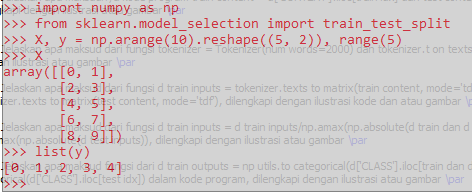
\includegraphics[width=0.5\textwidth]{figures/im/toke3.png}}
		\caption{For Train dan Test In Splits.}
		\label{toke3}
		\end{figure}

\item Jelaskan apa maksudnya kode program train content = d['CONTENT'].iloc[train idx] dan test content = d['CONTENT'].iloc[test idx]. dilengkapi dengan ilustrasi atau gambar \par
Code tersebut untuk mengambil data pada kolom atau index CONTENT yang merupakan bagian dari train\_idx dan test\_idx. Contoh sederhananya ketika data telah diubah menjadi data train dan data test maka kita dapat memilihnya untuk ditampilkan pada kolom yang diinginkan. Untuk ilustrasinya bisa dilihat pada gambar \ref{toke4}
		\begin{figure}[!htbp]
		\centerline{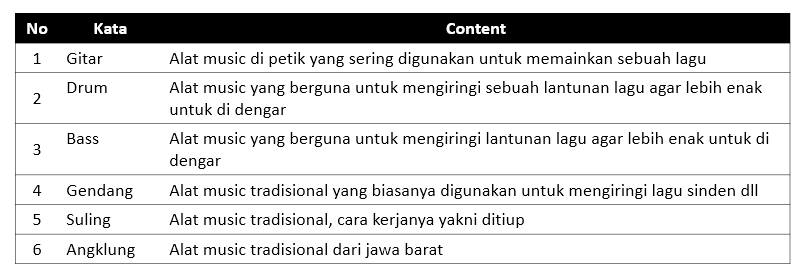
\includegraphics[width=0.5\textwidth]{figures/im/toke4.png}}
		\caption{Ilustrasi Content.}
		\label{toke4}
		\end{figure}

\item Jelaskan apa maksud dari fungsi tokenizer = Tokenizer(num words=2000) dan tokenizer fit on texts(train content), dilengkapi dengan ilustrasi atau gambar \par
Variabel tokenizer ini berfungsi untuk melakukan vektorisasi data kedalam bentuk token sebanyak 2000 kata. Dan selanjutnya akan melakukan fit tokenizer hanya untuk data training saja tidak dengan data testingnya. Untuk ilustrasinya bisa dilihat pada gambar \ref{toke5}
		\begin{figure}[!htbp]
		\centerline{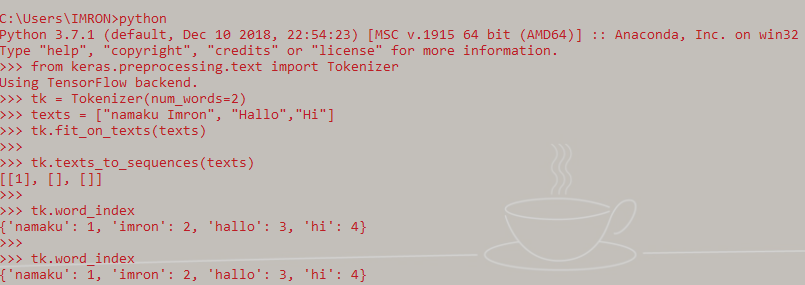
\includegraphics[width=0.5\textwidth]{figures/im/toke5.png}}
		\caption{Ilustrasi Fungsi Tokenizer.}
		\label{toke5}
		\end{figure}

\item Jelaskan apa maksud dari fungsi d train inputs = tokenizer.texts to matrix(train content, mode='tdf') dan d test inputs = tokenizer.texts to matrix(test content, mode='tdf'), dilengkapi dengan ilustrasi kode dan atau gambar \par
Code pertama yakni untuk merubah atau vektorisasi dari data training yang berupa teks menjadi matrix dengan menggunakan model tfidf. Code kedua sama halnya seperti yang pertama, yang membedakan hanya data yang dirubah. Untuk yang ini merubah data testing yang berupa teks menjadi matrix dengan menggunakan model tfidf. Ilustrasinya bisa dilihat pada gambar \ref{toke6}
		\begin{figure}[!htbp]
		\centerline{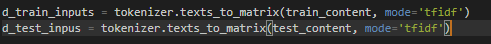
\includegraphics[width=0.5\textwidth]{figures/im/toke6.png}}
		\caption{Ilustrasi d\_train\_inputs.}
		\label{toke6}
		\end{figure}

\item Jelaskan apa maksud dari fungsi d train inputs = d train inputs/np.amax(np.absolute(d train dan d test inputs = d test inputs/np.amax(np.absolute(d test inputs)), dilengkapi dengan ilustrasi atau gambar \par
Code tersebut akan membagi matrix tfidf dengan amax yakni mengembalikan nilai maksimum array, dan hasilnya akan dimasukan kedalam variabel d train inputs untuk data train dan d test inputs untuk data testing dengan nominal absolut atau tanda adanya bilangan negatif dan koma. Ilustrasinya bisa dilihat pada gambar \ref{toke7}
		\begin{figure}[!htbp]
		\centerline{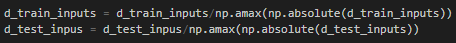
\includegraphics[width=0.5\textwidth]{figures/im/toke7.png}}
		\caption{Ilustrasi d\_train\_inputs.}
		\label{toke7}
		\end{figure}

\item Jelaskan apa maksud fungsi dari d train outputs = np utils.to categorical(d['CLASS'].iloc[train dan d test outputs = np utils.to categorical(d['CLASS'].iloc[test idx]) dalam kode program, dilengkapi dengan ilustrasi atau gambar \par
Code tersebut ditujukan untuk melakukan one-hot encoding agar dapat digunakan pada proses neural network. One-hot encoding tersebut diambil dari `CLASS' yang terdapat 2 neuron, yakni (1,0) dan (01) karena pilihannya hanya 2 yakni spam atau bukan spam.

\item Jelaskan apa maksud dari fungsi di listing 7.2. Gambarkan ilustrasi Neural Network nya dari model kode tersebut \par
\lstinputlisting[firstline=4, lastline=9]{src/ron/tujuh.py}
Code tersebut bertujuan untuk melakukan sequential, membandingkan setiap satu elemen dengan cara satu persatu secara beruntun. Dimana terdapat 512 neurons inputan dengan jumlah shape 2000 yang sebelumnya sudah dinormalisasi. Lalu model tersebut dilakukan aktivasi dengan menggunakan fungsi relu. Kemudian dilakukan pemotongan model tree sebesar 50\% agar tidak terjadi overfitting. Pada outputnya terdapat 2 neurons yakni (1,0) dan (0,1) yang akan di aktivasi dengan menggunakan fungsi softmax.

\item Jelaskan apa maksud dari fungsi di listing 7.3 dengan parameter tersebut \par
\lstinputlisting[firstline=11, lastline=11]{src/ron/tujuh.py}
Code tersebut akan melakukan compile model dengan fungsi optimizer, loss dan matrix.

\item Jelaskan apa itu Deep Learning \par
Deep Learning adalah salah satu cabang dari ilmu machine learning yang terdiri dari algoritma pemodelan abstraksi tingkat tinggi pada data menggunakan sekumpulan fungsi transformasi non-linear yang ditata berlapis-lapis dan mendalam. Teknik dan algoritma dalam machine learning dapat digunakan baik untuk supervised learning dan unsupervised learning.

\item Jelaskan apa itu Deep Neural Network, dan apa bedanya dengan Deep Learning \par
DNN adalah salah satu algoritma berbasis jaringan saraf tiruan yang memiliki dari 1 lapisan saraf tersembunyi yang dapat digunakan untuk pengambilan keputun. Perbedaannya dengan deep learning, yakni: DNN dapat menentukan dan mencerna karakteristik tertentu di suatu rangkaian data, kapabilitas lebih kompleks untuk mempelajari, mencerna, dan mengklasifikasikan data, serta dibagi ke dalam berbagai lapisan dengan fungsi yang berbeda-beda.

\item Jelaskan dengan ilustrasi gambar buatan sendiri(langkah per langkah) bagaimana perhitungan algoritma konvolusi dengan ukuran stride (NPM mod3+1) x (NPM mod3+1) yang terdapat max pooling \par
Konvolusi pada gambar dilakukan dalam image processing untuk menerapkan operator yang memiliki nilai output dari piksel gambar yang berasal dari kombinasi linear nilai input piksel, semakin nilai piksel tersebut maka kualitas gambar bisa semakin bagus. Untuk ilustrasinya bisa dilihat pada gambar \ref{toke13}
		\begin{figure}[!htbp]
		\centerline{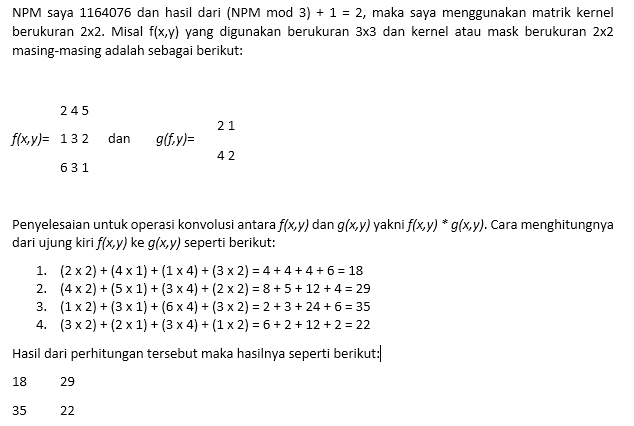
\includegraphics[width=0.5\textwidth]{figures/im/toke13.png}}
		\caption{Ilustrasi Algoritma Konvolusi.}
		\label{toke13}
		\end{figure}
\end{enumerate}


\section{Yusniar Nur Syarif Sidiq / 1164089}
\subsection{Teori / Yusniar Nur Syarif Sidiq / 1164089}
\begin{enumerate}

\item Jelaskan kenapa file teks harus di lakukan tokenizer. Dilengkapi dengan ilustrasi atau gambar !
	\subitem Sebelumnya kita harus tau terlebih dahulu apa itu Tokenizer, yaitu sebuah proses pembagian terhadap kalimat yang berada dalam dokumen sehingga menjadi sebuah bagian - bagian kata atau bisa kita sebut denga token. Dalam dataset Youtube Tokenizer digunakan untuk melakukan vektorisasi data, sehingga dapat kita simpulkan bahwa data yang telah kita buat dokumen pada chapter 6 yaitu data spam dan bukan spam akan dilakukan vektorisasi dengan menggunakan Tokenizer ini. Ilustrasi sederhana mengenai Tokenizer ini misalkan saya memiliki sebuah kalimat Nama Saya Adalah Yusniar jika gunakan fungsi Tokenizer ini akan dipecah menjadi kata per kata, perhatikan figure \ref{YNC7-1}.

	\begin{figure}[!htbp!]
		\centerline{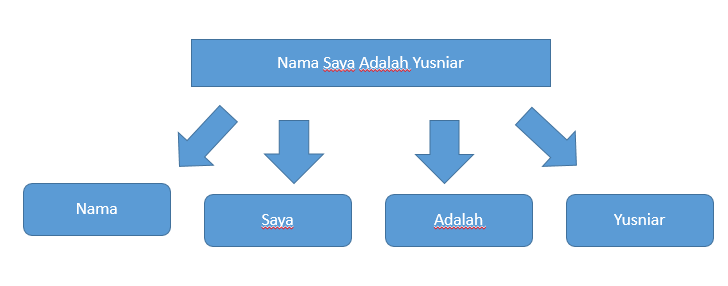
\includegraphics[width=0.5\textwidth]{figures/YN/Chapter7/YNC7-1.png}}
		\caption{Contoh Tokenizer.}
		\label{YNC7-1}
	\end{figure}

\item Jelaskan konsep dasar K Fold Cross Validation pada dataset komentar Youtube pada source code dibawah. Dilengkapi dengan ilustrasi atau gambar !
	\lstinputlisting[firstline=3, lastline=4]{src/yns/sc7.py}
	\subitem Pada variabel kfold berisikan StratifieldKFold yang dimana akan diisikan sebuah sempel dan dibagi menjadi 5 dengan nsplits pada setiap class. Lalu akan dibuat variabel baru yang dinamakan dengan 2splits dan disikan class dari dataset Youtube. Pada data yang telah dilakukan split akan diperoleh hasil presentase akhir. Ilustrasi yang saya berikan misalkan ada sebuah data lalu data tersebut akan dibagi menjadi data testing dan training lalu dilakukan fungsi Cross Validation untuk memperoleh hasil presentase akhir. Perhatikan figure \ref{YNC7-2}.

	\begin{figure}[!htbp!]
		\centerline{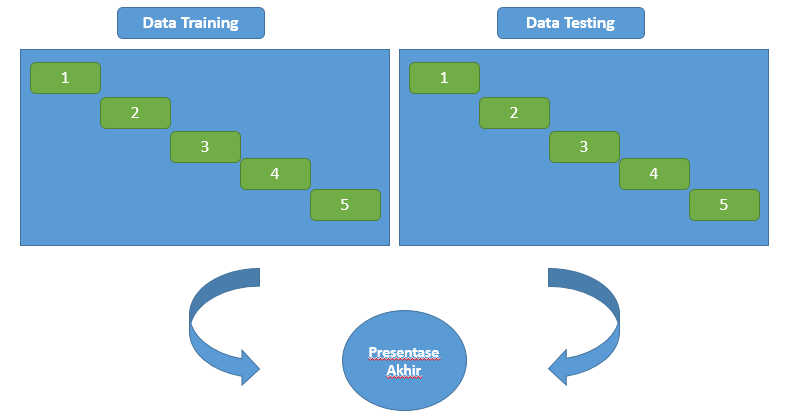
\includegraphics[width=0.5\textwidth]{figures/YN/Chapter7/YNC7-2.png}}
		\caption{Konsep Dasar K Fold Validation.}
		\label{YNC7-2}
	\end{figure}

\item Jelaskan apa maksudnya kode program for train, test in splits. Dilengkapi dengan ilustrasi atau gambar !
	\subitem Dimana fungsi tersebut digunakan untuk melakukan pengujian terhadap data yang sudah di split atau belum dalam dataset dan tidak akan terjadi penumpukan, maksudnya pada setiap class tidak akan menampilkan id yang sama. Kali ini saya akan memberikan ilustrasi sederhana, misalkan ada seseorang yang ingin menyumbangkan buku cerita kepada perpustakan, lalu pihak perpustakaan akan menerimanya, dikarenakan yang di sumbangkan adalah buku cerita dan bermacam - macam maka tidak akan ada buku yang sama hal ini sama saja bisa dibilang tidak adanya id yang sama. Untuk ilustrasi nya perhatikan figure \ref{YNC7-3}.

	\begin{figure}[!htbp!]
		\centerline{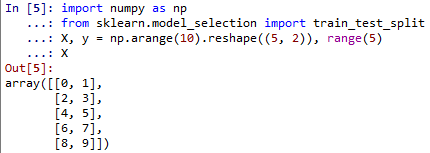
\includegraphics[width=0.5\textwidth]{figures/YN/Chapter7/YNC7-3.png}}
		\caption{Train And Test In Split.}
		\label{YNC7-3}
	\end{figure}

\item Jelaskan apa yang dimaksud kode program dibawah. Dilengkapi dengan ilustrasi atau gambar !
	\lstinputlisting[firstline=21, lastline=22]{src/yns/sc7.py}
	\subitem Dimana source code tersebut akan mengambil data dari kolom Content yaitu kolom tersebut merupakan bagian dari train\_idx dan test\_idx. Ilustrasi yang saya berikan yaitu apabila kita telah mengubah suatu data menjadi data training atau data testing maka kita dapat menampilkan data tersebut dengan isi kolom yang kita mau.

\item Jelaskan apa maksud dari fungsi tokenizer = Tokenizer(num\_words=2000) dan tokenizer.fit\_on\_texts(train\_content), dilengkapi ilustrasi atau gambar !
	\subitem Variabel tokenizer tersebut akan melakukan proses vektorisasi kata sebanyak 2000 kata dengan menggunakan fungsi Tokenizer. Pada source code tokenizer.fit\_on\_texts(train\_content) akan melakukan fit dengan menggunakan fungsi tokenizer akan tetapi hanya pada data training saja pada kolom content. Untuk ilustrasi dapat dilihat pada figure \ref{YNC7-4}

	\begin{figure}[!htbp!]
		\centerline{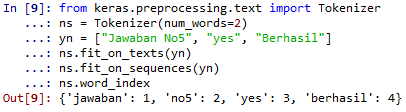
\includegraphics[width=0.5\textwidth]{figures/YN/Chapter7/YNC7-4.png}}
		\caption{Fungsi Tokenizer.}
		\label{YNC7-4}
	\end{figure}

\item Jelaskan apa yang dimaksud dari fungsi source code dibawah !
	\lstinputlisting[firstline=42, lastline=43]{src/yns/sc7.py}
	\subitem Pada source code baris pertama akan melakukan vektorisasi dari data training yang dimana data tersebut berbentuk string atau teks dan diubah kedalam bentuk matrix menggunakan model tdf. Untuk source code baris kedua akan melakukan vektorisasi data testing yang akan diubah kedalam bentuk matrix dengan mode tdf. Dimana kita ilustrasi source code nya adalah seperti yang ditampilkan pada figure \ref{YNC7-5}.

	\begin{figure}[!htbp!]
		\centerline{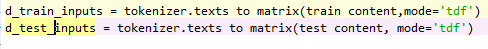
\includegraphics[width=0.5\textwidth]{figures/YN/Chapter7/YNC7-5.png}}
		\caption{Vektorisasi TDF Data Training Dan Testing.}
		\label{YNC7-5}
	\end{figure}

\item Jelaskan apa yang dimaksud dari fungsi d\_train\_inputs = d\_train\_inputs/np.amax(np.absolute(d\_train)) dan  d\_test\_inputs = d\_test\_inputs/np.amax(np.absolute(d\_test)), dilengkapi dengan ilustrasi atau gambar !
	\subitem Pada source code tersebut akan melakukan pembagian data matrix yang sudah kita buat pada data trainig dan testing dan akan mengembalikan nilai maksimum array menggunakan class amax. Untuk ilustrasi dapat dilihat pada figure \ref{YNC7-6}.

	\begin{figure}[!htbp!]
		\centerline{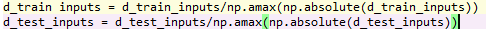
\includegraphics[width=0.5\textwidth]{figures/YN/Chapter7/YNC7-6.png}}
		\caption{Pembagian Data Matrix.}
		\label{YNC7-6}
	\end{figure}

\item Jelaskan apa yang dimaksud fungsi d\_train\_outputs = np\_utils.to\_categorical(d[CLASS].iloc[train\_idx] dan  d\_test\_outputs = np\_utils.to\_categorical(d[CLASS].iloc[test\_idx] dalam kode program dilengkapi dengan ilustrasi atau gamabar !
	\subitem Source code tersebut digunakan untuk melakuakan fungsi yang dinamakan One-hot encoding yang nantinya data tersebut dapat digunakan dalam proses Neural Network. Data yang diambil terdiri dari CLASS yaitu Spam dan No Spam dari data training dan data testing. Untuk ilustrasi dapat dilihat pada figure \ref{YNC7-7}.

	\begin{figure}[!htbp!]
		\centerline{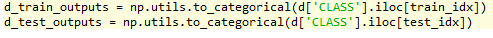
\includegraphics[width=0.5\textwidth]{figures/YN/Chapter7/YNC7-7.png}}
		\caption{One-hot Encoding.}
		\label{YNC7-7}
	\end{figure}

\item Jelaskan apa yang dimaksud dengan dari fungsi source code dibawah,
	\lstinputlisting[firstline=8, lastline=13]{src/yns/sc7.py}
	\subitem Source Code tersebut akan melakukan sequential yang diamana akan melakukan perbandingan pada setiap elemen secara satu persatu dan berurut. Terdapat 512 Neurons dengan jumlah input shape sebesar 2000 yang dimana sudah dilakukan normalisasi. Mpdel tersebut akan dilakukan aktivasi menggunakan model relu lalu dilakukan dropout atau pemotongan sebesar 50\%. Pada neurons selanjutnya terdapat 2  yang kemudian akan dilakukan aktivasi menggunakan fungsi softmax.

\item Jelaskan apa yang dimaksud dari fungsi pada source code dibawah dengan parameter tersebut !
	\lstinputlisting[firstline=17, lastline=17]{src/yns/sc7.py}
	\subitem Source code tersebut akan melakukan proses compile dengan menggunakan fungsi optimizer dan memunculkan data loss dan akurasi matrix.

\item Jelaskan apa itu Deep Learning !
	\subitem Deep Learning merupakan sebuah cabang dari Mechine Learning dimana konesep yang deep learning ini hampir serupa dengan Mechine Learning hanya saja deep learning dilakukan dengan metode yang lebih cerdas, contohnya dalam menditeksi wajah itu termasuk deep learning.

\item Jelaskan apa itu Deep Neural Network dan apa bedanya dengan Deep Learning !
	\subitem Deep Neural Network merupakan sebuah algoritma berbasis Neural Netowork yang digunakan dalam pengambilan sebuah keputusan. Perbedaan DNN dengan DL antara lain DNN merupakan algoritma yang digunakan terhadap DL sedangkan DL yang akan menggunakan algoritma tersebut.

\item Jelaskan dengan ilustrasi gambar langkah per langkah bagaimana perhitungan algoritma konvolusi dengan ukuran stide (NPM mod 3 + 1) x (NPM mod 3 + 1) yang terdapat max pooling !

	\begin{itemize}
		\item Pertama tentukan nilai (x,y) dan (x1,y1)
		\item Nilai tersebut dibuat kedalam bentuk matrix
		\item Jika sudah berbentuk matrix lakukan perkalian antar baris dan deret
		\item Hasil perkalian tersebut dijumlahkan sehingga akan menghasilkan nilai matrix (3x3)
	\end{itemize}

	\subitem Untuk ilustrasi dapat dilihat pada figure \ref{YNC7-8}

	\begin{figure}[!htbp!]
		\centerline{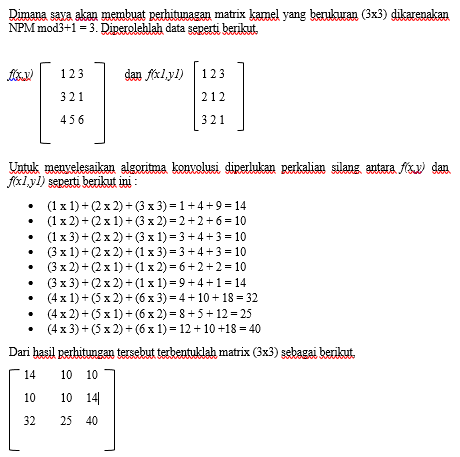
\includegraphics[width=0.5\textwidth]{figures/YN/Chapter7/YNC7-8.png}}
		\caption{Algoritma Konvolusi Dengan Matrix (3x3).}
		\label{YNC7-8}
	\end{figure}	

\end{enumerate}

\subsection{Keterampilam Pemrograman}
\begin{enumerate}

\item Jelaskan kode program pada blok \# In[1]. Jelaskan arti dari setiap baris kode yang dibuat dan hasi keliarannya dari komputer sendiri !
	\lstinputlisting[firstline=1, lastline=4]{src/yns/YNC7.py}
	\subitem Hasil dari source code tersebut dapat dilihat pada figure \ref{YNC7-9}
	\begin{figure}[!htbp!]
		\centerline{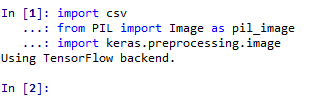
\includegraphics[width=0.5\textwidth]{figures/YN/Chapter7/YNC7-9.png}}
		\caption{Source Code 1}
		\label{YNC7-9}
	\end{figure}	

\item Jelaskan kode program pada blok \# In[2]. Jelaskan arti dari setiap baris kode yang dibuat dan hasi keliarannya dari komputer sendiri !
	\lstinputlisting[firstline=6, lastline=19]{src/yns/YNC7.py}
	\subitem Hasil dari source code tersebut dapat dilihat pada figure \ref{YNC7-10}
	\begin{figure}[!htbp!]
		\centerline{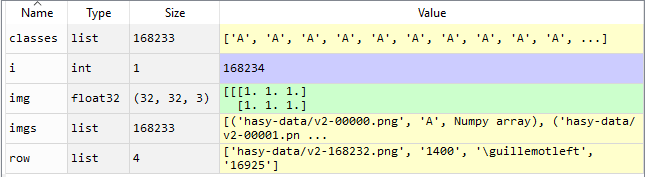
\includegraphics[width=0.5\textwidth]{figures/YN/Chapter7/YNC7-10.png}}
		\caption{Source Code 2}
		\label{YNC7-10}
	\end{figure}	

\item Jelaskan kode program pada blok \# In[3]. Jelaskan arti dari setiap baris kode yang dibuat dan hasi keliarannya dari komputer sendiri !
	\lstinputlisting[firstline=21, lastline=26]{src/yns/YNC7.py}
	\subitem Hasil dari source code tersebut dapat dilihat pada figure \ref{YNC7-11}
	\begin{figure}[!htbp!]
		\centerline{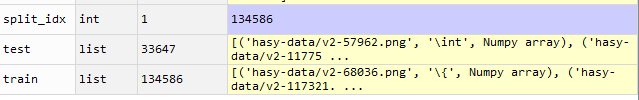
\includegraphics[width=0.5\textwidth]{figures/YN/Chapter7/YNC7-11.png}}
		\caption{Source Code 3}
		\label{YNC7-11}
	\end{figure}	

\item Jelaskan kode program pada blok \# In[4]. Jelaskan arti dari setiap baris kode yang dibuat dan hasi keliarannya dari komputer sendiri !
	\lstinputlisting[firstline=30, lastline=36]{src/yns/YNC7.py}
	\subitem Hasil dari source code tersebut dapat dilihat pada figure \ref{YNC7-12}
	\begin{figure}[!htbp!]
		\centerline{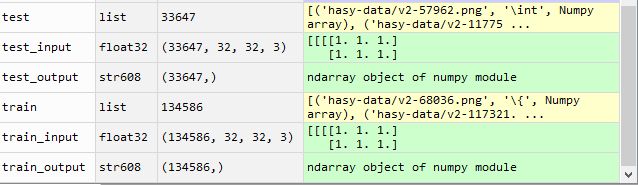
\includegraphics[width=0.5\textwidth]{figures/YN/Chapter7/YNC7-12.png}}
		\caption{Source Code 4}
		\label{YNC7-12}
	\end{figure}	

\item Jelaskan kode program pada blok \# In[5]. Jelaskan arti dari setiap baris kode yang dibuat dan hasi keliarannya dari komputer sendiri !
	\lstinputlisting[firstline=39, lastline=40]{src/yns/YNC7.py}
	\subitem Hasil dari source code tersebut dapat dilihat pada figure \ref{YNC7-13}
	\begin{figure}[!htbp!]
		\centerline{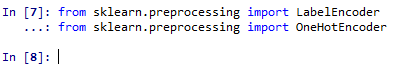
\includegraphics[width=0.5\textwidth]{figures/YN/Chapter7/YNC7-13.png}}
		\caption{Source Code 5}
		\label{YNC7-13}
	\end{figure}	

\item Jelaskan kode program pada blok \# In[6]. Jelaskan arti dari setiap baris kode yang dibuat dan hasi keliarannya dari komputer sendiri !
	\lstinputlisting[firstline=44, lastline=46]{src/yns/YNC7.py}
	\subitem Hasil dari source code tersebut dapat dilihat pada figure \ref{YNC7-14}
	\begin{figure}[!htbp!]
		\centerline{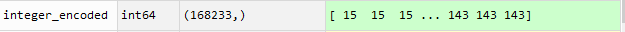
\includegraphics[width=0.5\textwidth]{figures/YN/Chapter7/YNC7-14.png}}
		\caption{Source Code 6}
		\label{YNC7-14}
	\end{figure}	

\item Jelaskan kode program pada blok \# In[7]. Jelaskan arti dari setiap baris kode yang dibuat dan hasi keliarannya dari komputer sendiri !
	\lstinputlisting[firstline=49, lastline=54]{src/yns/YNC7.py}
	\subitem Hasil dari source code tersebut dapat dilihat pada figure \ref{YNC7-15}
	\begin{figure}[!htbp!]
		\centerline{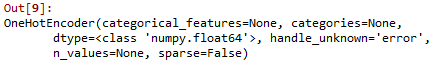
\includegraphics[width=0.5\textwidth]{figures/YN/Chapter7/YNC7-15.png}}
		\caption{Source Code 7}
		\label{YNC7-15}
	\end{figure}	

\item Jelaskan kode program pada blok \# In[8]. Jelaskan arti dari setiap baris kode yang dibuat dan hasi keliarannya dari komputer sendiri !
	\lstinputlisting[firstline=57, lastline=68]{src/yns/YNC7.py}
	\subitem Hasil dari source code tersebut dapat dilihat pada figure \ref{YNC7-16}
	\begin{figure}[!htbp!]
		\centerline{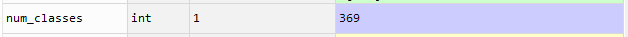
\includegraphics[width=0.5\textwidth]{figures/YN/Chapter7/YNC7-16.png}}
		\caption{Source Code 8}
		\label{YNC7-16}
	\end{figure}	

\item Jelaskan kode program pada blok \# In[9]. Jelaskan arti dari setiap baris kode yang dibuat dan hasi keliarannya dari komputer sendiri !
	\lstinputlisting[firstline=71, lastline=76]{src/yns/YNC7.py}
	\subitem Hasil dari source code tersebut dapat dilihat pada figure \ref{YNC7-17}
	\begin{figure}[!htbp!]
		\centerline{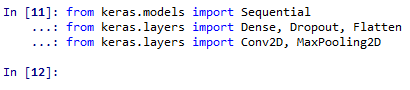
\includegraphics[width=0.5\textwidth]{figures/YN/Chapter7/YNC7-17.png}}
		\caption{Source Code 9}
		\label{YNC7-17}
	\end{figure}	

\item Jelaskan kode program pada blok \# In[10]. Jelaskan arti dari setiap baris kode yang dibuat dan hasi keliarannya dari komputer sendiri !
	\lstinputlisting[firstline=78, lastline=103]{src/yns/YNC7.py}
	\subitem Hasil dari source code tersebut dapat dilihat pada figure \ref{YNC7-18}
	\begin{figure}[!htbp!]
		\centerline{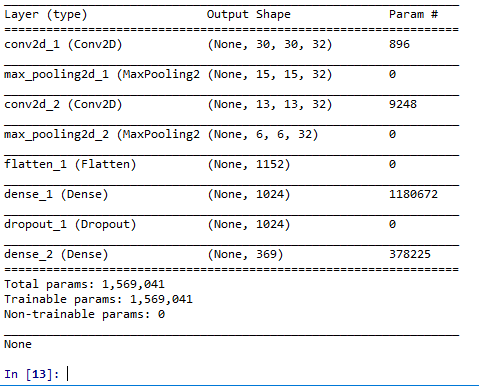
\includegraphics[width=0.5\textwidth]{figures/YN/Chapter7/YNC7-18.png}}
		\caption{Source Code 10}
		\label{YNC7-18}
	\end{figure}

\item Jelaskan kode program pada blok \# In[11]. Jelaskan arti dari setiap baris kode yang dibuat dan hasi keliarannya dari komputer sendiri !
	\lstinputlisting[firstline=106, lastline=109]{src/yns/YNC7.py}
	\subitem Hasil dari source code tersebut dapat dilihat pada figure \ref{YNC7-19}
	\begin{figure}[!htbp!]
		\centerline{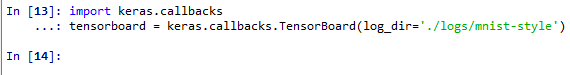
\includegraphics[width=0.5\textwidth]{figures/YN/Chapter7/YNC7-19.png}}
		\caption{Source Code 11}
		\label{YNC7-19}
	\end{figure}

\item Jelaskan kode program pada blok \# In[12]. Jelaskan arti dari setiap baris kode yang dibuat dan hasi keliarannya dari komputer sendiri !
	\lstinputlisting[firstline=111, lastline=122]{src/yns/YNC7.py}
	\subitem Hasil dari source code tersebut dapat dilihat pada figure \ref{YNC7-20}
	\begin{figure}[!htbp!]
		\centerline{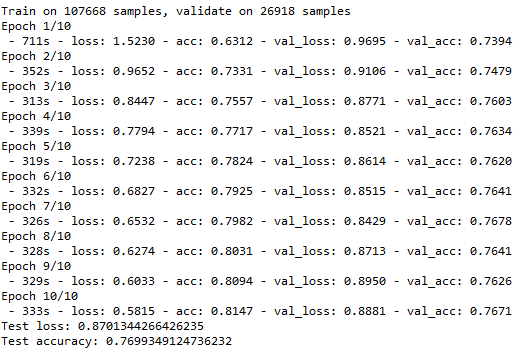
\includegraphics[width=0.5\textwidth]{figures/YN/Chapter7/YNC7-20.png}}
		\caption{Source Code 12}
		\label{YNC7-20}
	\end{figure}

\item Jelaskan kode program pada blok \# In[13]. Jelaskan arti dari setiap baris kode yang dibuat dan hasi keliarannya dari komputer sendiri !
	\lstinputlisting[firstline=126, lastline=171]{src/yns/YNC7.py}
	\subitem Hasil dari source code tersebut dapat dilihat pada figure \ref{YNC7-21}
	\begin{figure}[!htbp!]
		\centerline{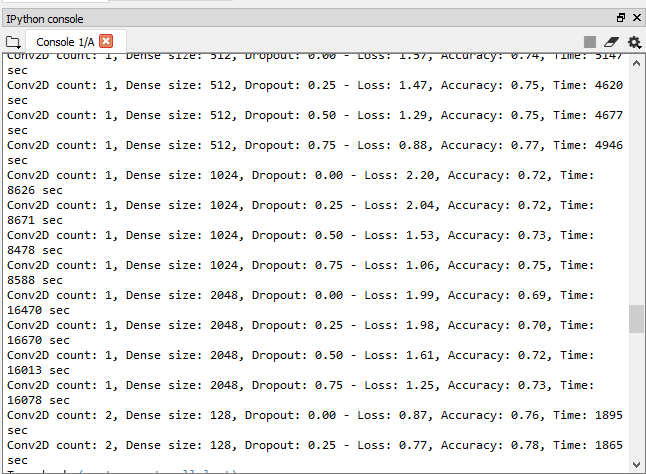
\includegraphics[width=0.5\textwidth]{figures/YN/Chapter7/YNC7-21.png}}
		\caption{Source Code 13}
		\label{YNC7-21}
	\end{figure}

\item Jelaskan kode program pada blok \# In[14]. Jelaskan arti dari setiap baris kode yang dibuat dan hasi keliarannya dari komputer sendiri !
	\lstinputlisting[firstline=174, lastline=197]{src/yns/YNC7.py}
	\subitem Hasil dari source code tersebut dapat dilihat pada figure \ref{YNC7-22}
	\begin{figure}[!htbp!]
		\centerline{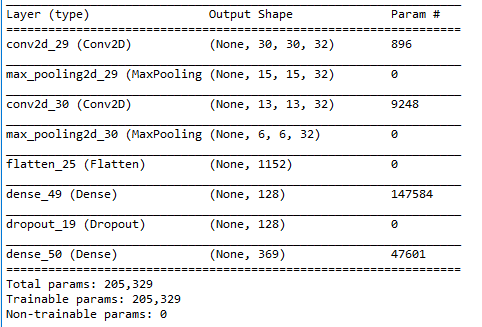
\includegraphics[width=0.5\textwidth]{figures/YN/Chapter7/YNC7-22.png}}
		\caption{Source Code 14}
		\label{YNC7-22}
	\end{figure}

\item Jelaskan kode program pada blok \# In[15]. Jelaskan arti dari setiap baris kode yang dibuat dan hasi keliarannya dari komputer sendiri !
	\lstinputlisting[firstline=198, lastline=203]{src/yns/YNC7.py}
	\subitem Hasil dari source code tersebut dapat dilihat pada figure \ref{YNC7-23}
	\begin{figure}[!htbp!]
		\centerline{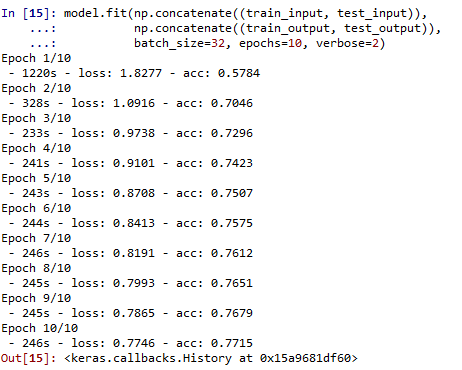
\includegraphics[width=0.5\textwidth]{figures/YN/Chapter7/YNC7-23.png}}
		\caption{Source Code 15}
		\label{YNC7-23}
	\end{figure}

\item Jelaskan kode program pada blok \# In[16]. Jelaskan arti dari setiap baris kode yang dibuat dan hasi keliarannya dari komputer sendiri !
	\lstinputlisting[firstline=205, lastline=207]{src/yns/YNC7.py}
	\subitem Hasil dari source code tersebut dapat dilihat pada figure \ref{YNC7-24}
	\begin{figure}[!htbp!]
		\centerline{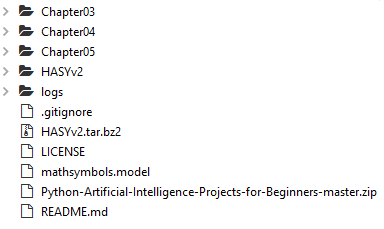
\includegraphics[width=0.5\textwidth]{figures/YN/Chapter7/YNC7-24.png}}
		\caption{Source Code 16}
		\label{YNC7-24}
	\end{figure}

\item Jelaskan kode program pada blok \# In[17]. Jelaskan arti dari setiap baris kode yang dibuat dan hasi keliarannya dari komputer sendiri !
	\lstinputlisting[firstline=209, lastline=211]{src/yns/YNC7.py}
	\subitem Hasil dari source code tersebut dapat dilihat pada figure \ref{YNC7-25}
	\begin{figure}[!htbp!]
		\centerline{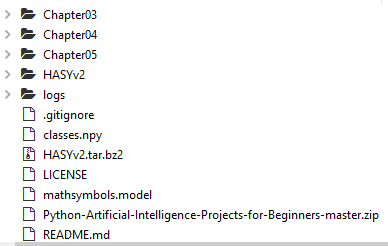
\includegraphics[width=0.5\textwidth]{figures/YN/Chapter7/YNC7-25.png}}
		\caption{Source Code 17}
		\label{YNC7-25}
	\end{figure}

\item Jelaskan kode program pada blok \# In[18]. Jelaskan arti dari setiap baris kode yang dibuat dan hasi keliarannya dari komputer sendiri !
	\lstinputlisting[firstline=214, lastline=220]{src/yns/YNC7.py}
	\subitem Hasil dari source code tersebut dapat dilihat pada figure \ref{YNC7-26}
	\begin{figure}[!htbp!]
		\centerline{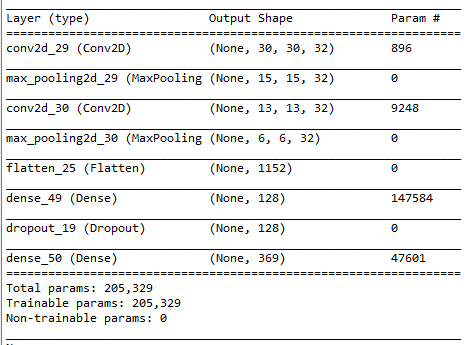
\includegraphics[width=0.5\textwidth]{figures/YN/Chapter7/YNC7-26.png}}
		\caption{Source Code 18}
		\label{YNC7-26}
	\end{figure}

\item Jelaskan kode program pada blok \# In[19]. Jelaskan arti dari setiap baris kode yang dibuat dan hasi keliarannya dari komputer sendiri !
	\lstinputlisting[firstline=222, lastline=239]{src/yns/YNC7.py}
	\subitem Hasil dari source code tersebut dapat dilihat pada figure \ref{YNC7-27}
	\begin{figure}[!htbp!]
		\centerline{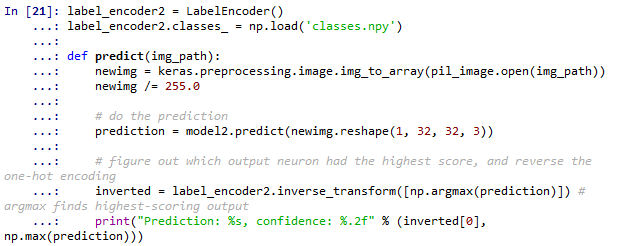
\includegraphics[width=0.5\textwidth]{figures/YN/Chapter7/YNC7-27.png}}
		\caption{Source Code 19}
		\label{YNC7-27}
	\end{figure}

\item Jelaskan kode program pada blok \# In[20]. Jelaskan arti dari setiap baris kode yang dibuat dan hasi keliarannya dari komputer sendiri !
	\lstinputlisting[firstline=241, lastline=247]{src/yns/YNC7.py}
	\subitem Hasil dari source code tersebut dapat dilihat pada figure \ref{YNC7-28}
	\begin{figure}[!htbp!]
		\centerline{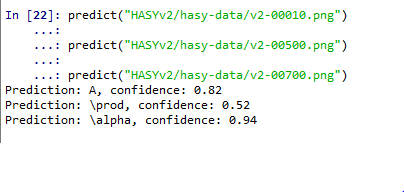
\includegraphics[width=0.5\textwidth]{figures/YN/Chapter7/YNC7-28.png}}
		\caption{Source Code 20}
		\label{YNC7-28}
	\end{figure}

\end{enumerate}

\subsection{Penanganan Error}
\begin{enumerate}

\item Dari Praktek pemrograman yang dilakukan di modul ini, error yang kita dapatkan di dokumentasikan dan di selesaikan !
	\begin{itemize}

	\item Screenshoot Error, dapat dilihat pada figure \ref{YNC7-29}
	
	\begin{figure}[!htbp!]
		\centerline{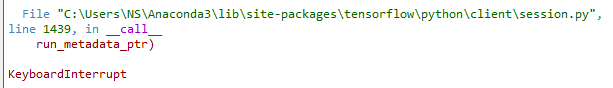
\includegraphics[width=0.5\textwidth]{figures/YN/Chapter7/YNC7-29.png}}
		\caption{Error Yang Di Dapatkan}
		\label{YNC7-29}
	\end{figure}

	\item Tuliskan source code error dan jenis errornya,
	\lstinputlisting[firstline=250, lastline=251]{src/yns/YNC7.py}

	\item Solusi pemecahan masalah error tersebut, dimana kita harus menunggu hingga program selesai berjalan sehingga menciptakan hasil yang maksimal pada saat kita tentukan prediksinya.
		
	\end{itemize}

\end{enumerate}